\begin{figure}[h!]
    \centering
    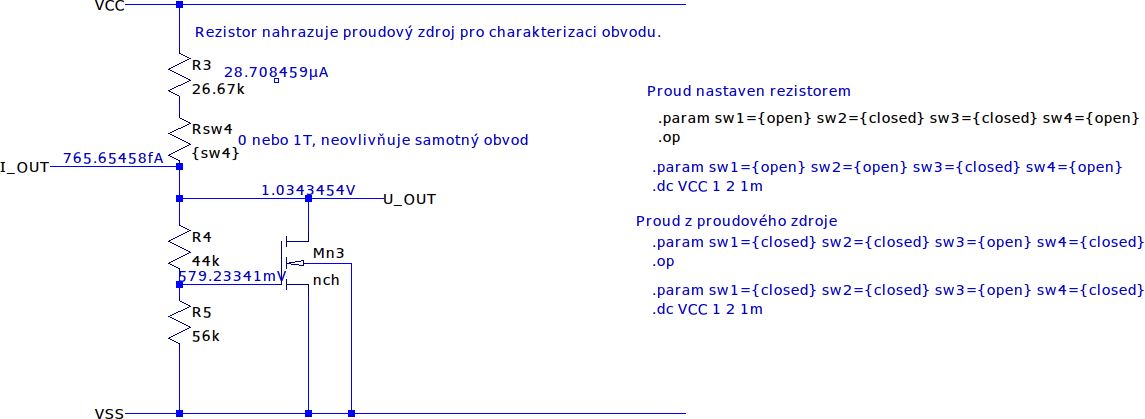
\includegraphics[scale=0.5]{spice2-1.png}
    \caption{Napěťová reference, analýza OP -- proud přes rezistor.}
    \label{fig:spice0-png}
  \end{figure}

  \begin{figure}[h!]
    \centering
    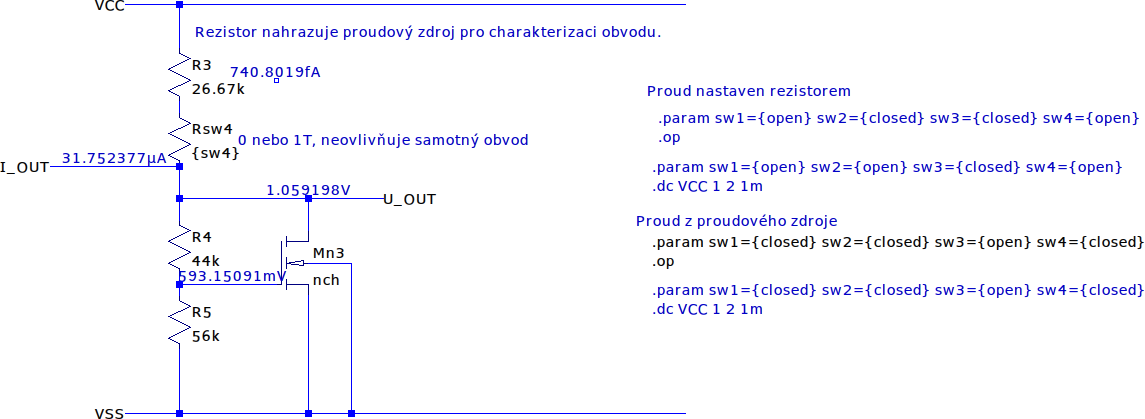
\includegraphics[scale=0.5]{spice2-2.png}
    \caption{Napěťová reference, analýza OP -- proud z proud. reference.}
    \label{fig:spice0-png}
  \end{figure}


\clearpage
\subsubsection{Ruční návrh}
Proud z proudového zdroje se rozdělí do dvou větví, tranzistorem necháme procházet větší část, konkrétně \qty{20}{\micro\ampere}, pro jeho rozměry pak platí:
Nejprve vypočítám rozměry pro tranzistor \(M_{N3} \):
\[
    \frac{W_{N3} }{L}=\frac{2\cdot I_{D}}{KP_{N}\cdot (U_{GS} -U_{TH})^2 } 
\]
\[
    \frac{W_{N3} }{L}=\frac{2\cdot \num{20e-6}}{\num{220e-6}\cdot (\num{0.2})^2 } 
\]

\[
    \frac{W_{N3} }{L}\doteq \num[round-mode=places,round-precision=2]{4.545454545454545} 
\]
Délku \(L\) zvolíme opět \qty{2}{\micro\meter}, tedy \(W_{N3}= \qty{9.09}{\micro\meter}\). 

Odporovou větví tedy prochází proud \(I_{R} =\qty{10}{\micro\ampere}\), který na rezistoru \(R_{5} \) tvoří úbytek napětí rovný napětí \(U_{GS} \) tranzistoru. Pro hodnoty rezitorů platí:
\begin{align*}
    R_{5} =& \frac{U_{R5}}{I_{R}} \\
          =& \frac{U_{GS,MN3}}{I_{R}} \\
          =& \frac{U_{TH0,N3}+U_{OV,N3} }{I_{R}} \\
          =& \frac{\num{360e-3}+\num{0.2} }{\num{10e-6}} \\
          =& \qty{56}{\kilo\ohm}
\end{align*}
\begin{align*}
    R_{4} =& \frac{U_{REF}}{I_{R}} - R_{1}  \\
          =& \frac{1}{\num{10e-6}} - \num{56e3}  \\
          =& \qty{44}{\kilo\ohm}
\end{align*}
Pro nastavení proudu použjeme rezistor \(R_{3} \):
\begin{align*}
    R_{3} =& \frac{U_{CC} - U_{REF}}{\num{30e-6}}  \\
          =& \frac{\num{1.8} - 1}{\num{30e-6}}  \\
          =& \qty{26.67}{\kilo\ohm}
\end{align*}




\subsubsection{Simulace}

\begin{figure}[h!]
    \centering
    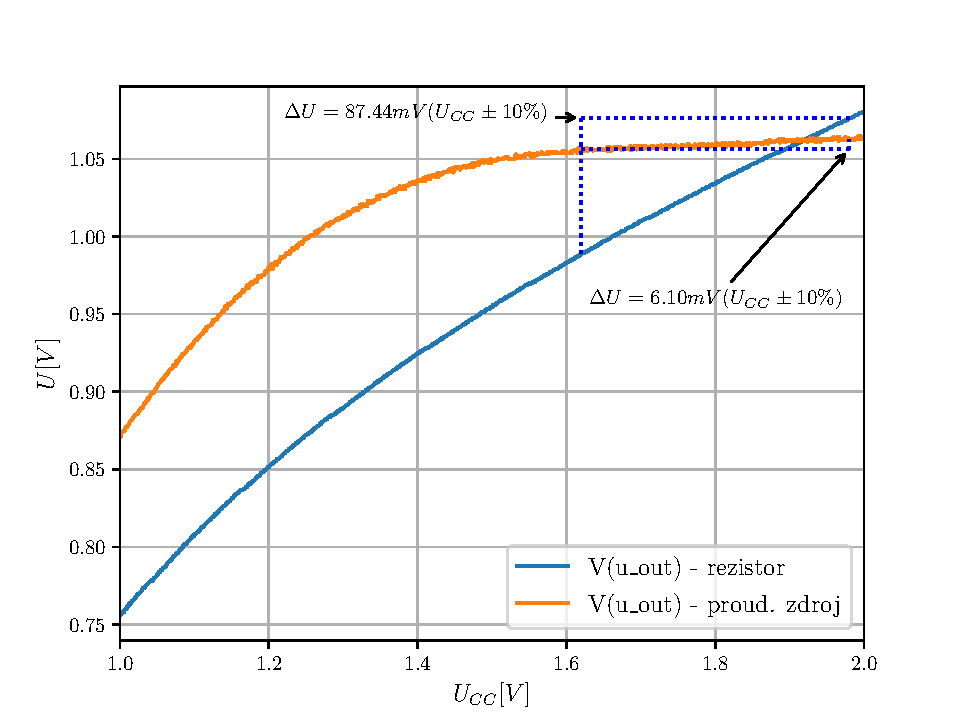
\includegraphics[width=0.8\textwidth]{img/3-2-3.pdf}
    \caption{Časová analýza -- srovnání výstupů napěťové reference.}
    \label{fig:img/3-2-3.pdf}
\end{figure}